\documentclass[a4paper,10pt]{article}
\usepackage[utf8]{inputenc}
\usepackage[margin=0.8in]{geometry}
\usepackage{graphicx}
\usepackage[english]{isodate}
\usepackage[document]{ragged2e}
\graphicspath{ {./img/} }
\usepackage{amsmath}
\usepackage{makecell}
\usepackage{longtable}
\usepackage{hyperref}
\usepackage{url}
\usepackage{textcomp}


\title{DSGA1011 Homework 2: RNN/CNN-based Natural Language Inference}
\author{Rong Feng - rf1316}
\date{\printdayoff\today}

\begin{document}

%\maketitle
Rong Feng, rf1316, Oct 2018, DS-GA1011 HW2: RNN/CNN-based Natural Language Inference \\ 
Public GitHub: \footnote{\url{https://github.com/rmfeng/ds1011_public/tree/master/hw2}}\\
Since this assignment tackles the bonus section of fine tuning the models, it has a page limit of 6 pages.

\section{Summary}
\par 
\justify
In part 1 of this assignemnt, both RNN and CNN architectures are used to tackle the Stanford NLI classification problem \cite{nlistanford}. The best validation accuracy under the RNN architecture achieved 74.0\% and under the CNN architecture achieved 70.3\% The hyperparameters used are summarized in Table \ref{tbl:finalhparams} below. In part 2, the best RNN model was used to first evaluate each genre in the MNLI dataset, and then subsequently tuned for another 5 epochs at a reduced learning rate and smaller batch size. The results before and after tuning are summarized in Table \ref{tbl:mnliresults}. The Avg Cross Genre column represents the average accuracy for that genre's post tune model when used to validate all of other genres.

\par
\justify
The final RNN model ran for roughly 30mins on 1 GPU and early stopped in the 3rd epoch. The final CNN model ran for roughly 20mins on 1 GPU and also early stopped in the 3rd epoch


\begin{table}[!htbp]
\begin{tabular}{| l | l | l | l |}
\hline
Hyperparameter   & Description                                & Final RNN Model     & Final CNN Model \\
\hline
LR               & Learning Rate on used Optimizer            & 0.01      & 0.001     \\
LR\_DECAY\_RATE  & Gamma decay rate per epoch                 & 0.95      & 0.95      \\
NEPOCH           & Max number of Epochs                       & 10        & 10      \\
VOC\_SIZE        & Vocab Size                                 & 100k      & 100k     \\
HIDDEN\_DIM      & RNN / CNN hidden dimension                 & 100       & 200   \\
BATCH\_SIZE      & Batch size                                 & 256       & 256   \\
DROP\_OUT\_RNN   & Dropout in the RNN layers                  & 0.25      & N/A   \\
DROP\_OUT\_FC    & Dropout in the fully-connected layers      & 0.25      & 0.5   \\
CNN\_KERN\_SIZE  & Kernal size for the CNN, pad = (K-1)/2     & N/A       & 3      \\
EARLY\_STOP      & Whether to consider early stop             & True      & True     \\
ES\_LOOKBACK     & \# of steps to look back for early stop    & 50        & 50     \\
NI\_DECREASE\_LR & If no improvement, reduce LR by factor     & True      & True     \\
NI\_LOOKBACK     & \# of steps to look back for improvement   & 25        & 25     \\
OPTIMIZER        & PyTorch Optimizer Used                     & Adam      & Adam     \\
\hline
\end{tabular}
\caption{Final Hyperparameters}\label{tbl:finalhparams}
\end{table}


\begin{table}[!htbp]
\begin{tabular}{| l | l | l | l | l |}
\hline
Genre      & Pre-tuning(CNN) & Pre-tuning(RNN) & Post-tuning(RNN) & Avg Cross Genre \\
\hline
fiction    & 45.8\%   & 49.0\%   & 58.8\%   & 50.7\%    \\
\hline
telephone  & 46.5\%   & 50.0\%   & 57.9\%   & 52.4\%    \\
\hline
slate      & 43.1\%   & 47.6\%   & 49.7\%   & 52.5\%    \\
\hline
government & 43.5\%   & 50.7\%   & 61.1\%   & 52.2\%    \\
\hline
travel     & 46.5\%   & 47.9\%   & 55.9\%   & 50.0\%    \\
\hline
\end{tabular}
\caption{MNLI Results}\label{tbl:mnliresults}
\end{table}

\par
\justify
Correct Answers:
\begin{itemize}
\item Example 1
	\begin{itemize}
	\item Sentence 1: four people sit on a subway two read books , one looks at a cellphone and is wearing knee high boots
	\item Sentence 2: multiple people are on a subway together , with each of them doing their own thing
	\item Label: entailment
	\item Prediction: entailment
	\item Explanation: The model correctly identifies that four is the same as multiple people, and that the remaining words in sentence 1 is describing the actions of each person.
	\end{itemize}
\end{itemize}

\begin{itemize}
\item Example 2
	\begin{itemize}
	\item Sentence 1: bicycles stationed while a group of people socialize
	\item Sentence 2: people get together near a stand of bicycles
	\item Label: entailment
	\item Prediction: entailment
	\item Explanation: The model correctly determines that the flipped nature of the two sentances do not contradict each other, likely a benefit of the bi-directional GRUs
	\end{itemize}
\end{itemize}

\begin{itemize}
\item Example 3
	\begin{itemize}
	\item Sentence 1: man in overalls with two horses
	\item Sentence 2: a man in overalls with two horses
	\item Label: entailment
	\item Prediction: entailment
	\item Explanation: This was an easy one, the 2 sentences are almost identical
	\end{itemize}
\end{itemize}

\par
\justify
Incorrect Answers:
\begin{itemize}
\item Example 1
	\begin{itemize}
	\item Sentence 1: three women on a stage , one wearing red shoes , black pants , and a gray shirt is sitting on a prop , another is sitting on the floor , and the third wearing a black shirt and pants is standing , as a gentleman in the back tunes an instrument
	\item Sentence 2: there are two women standing on the stage 
	\item Label: contradiction
	\item Prediction: entailment
	\item Explanation: It is hard for the model to recognize the fact that 2 of them are not standing. The model probably flagged as entailment as all three of them are indeed on the stage.
	\end{itemize}
\end{itemize}

\begin{itemize}
\item Example 2
	\begin{itemize}
	\item Sentence 1: two people are in a green forest
	\item Sentence 2: the forest is not dead
	\item Label: entailment
	\item Prediction: contradiction
	\item Explanation: The sentences were very short, with the only link being the forest. The 2nd sentence can be interpreted in many different ways. Even for a human, this sentence pair would be hard to classify.
	\end{itemize}
\end{itemize}

\begin{itemize}
\item Example 3
	\begin{itemize}
	\item Sentence 1: two women , one walking her dog the other pushing a stroller
	\item Sentence 2: there is a snowstorm
	\item Label: contradiction
	\item Prediction: neutral
	\item Explanation: To make this inference, the model would have to imply that walking a dog implies outside and pushing a stroller implies a higher care for not doing so when there is inclement weather. Due the the several stages of implications, it would be hard for the model to make that call. However, the neutral prediction isn't so bad, as the two sentences do have very little overlap.
	\end{itemize}
\end{itemize}


\section{RNN Architecture}
For the RNN, the graph stack this:
\begin{itemize}
\item Pretrained Embedding (frozen)
\item Single-layered bi-directional GRU for sentence 1
\item In parallel: single-layered bi-directional GRU for sentence 2
\item Concatenation of final hidden states in the 2 GRUs
\item Linear(Input Size: 2x hidden state size, Output Size: FC\_HIDDEN hyperparameter)
\item ReLU
\item Linear(Input Size: FC\_HIDDEN, Output Size: number of classes)
\item Softmax classifier
\end{itemize}

\section{CNN Architecture}
For the CNN, the graph stack is:
\begin{itemize}
\item Pretrained Embedding (frozen)
\item For Sentence 1 a CNN Graph:
\begin{itemize}
	\item 1-D Convolution (Kernal Size = CNN\_KERN\_SIZE hyperparameter, Padding = (K - 1) /2), this layer takes the embedding size as input and convolves it to HIDDEN\_DIM size
	\item ReLU
	\item 1-D Convolution (Kernal Size = CNN\_KERN\_SIZE hyperparameter, Padding = (K - 1) /2), this layer takes the HIDDEN\_DIM as input and convolves it to the same size 
	\item Maxpool on time dimesion
\end{itemize}
\item In parallel: same CNN graph for sentence 2
\item Concatenation of final states in the 2 CNNs
\item Linear(Input Size: 2x hidden state size, Output Size: FC\_HIDDEN hyperparameter)
\item ReLU
\item Linear(Input Size: FC\_HIDDEN, Output Size: number of classes)
\item Softmax classifier
\end{itemize}


\section{Data Preparation}

\par 
\justify
\textbf{Loading pretrained word Vectors:} the wikinews 300d 1 million word vectors were downloaded from the FastText website \cite{fasttext} and loaded in a frozen state to be used in the embedding layer. The VOC\_SIZE hyperparameter determined how many words from this pretrained set to use to build our vocabulary, in addition to the $<$pad$>$ and $<$unk$>$ characters at index 0 and 1 respectively.

\par 
\justify
\textbf{Loading the SNLI Data:} 100k rows were found in the SNLI training dataset and 1000 in the SNLI validation dataset, no test dataset was used. The data was loaded into a custom SNLIDatum class and then subsequently piped into a pytorch DataLoader. The tokenization was simply space delimit and each token was mapped to the appropriate row in the pretrained universe. Any unknown words was mapped to a $<$unk$>$ character with a randomly initialized word vector that had the same standard deviation as the FastText ones, and normally distributed around 0. Finally, a collate function was provided for the pytorch DataLoader class and the training data was set to shuffle while the validation data was not.

\par 
\justify
\textbf{Loading the MNLI Data:} The same loader was used for MNLI with the exception that any rows with genres not equal to the specified one was ignored. Additionally there was 1 sentence in the mnli validation set that was of length greater than 10000, that looks like to be an error. This record was ignored for all loaders.

\section{RNN Hyperparameter Grid Search}
A basic grid search was performed for RNNs over the following parameter permutations: 
\begin{itemize}
\item Learning Rate: [0.01, 0.001]
\item Learning Rate Decay Per Epoch: [0.95, 0.8]
\item RNN Hidden Size: [50, 100, 200]
\item RNN and FC Dropout Rate: [0.25, 0.5, 0.75]
\end{itemize}

\par 
\justify
These permutations gave us a total of 36 training instances of which the best model was chosen to be the final RNN model. The training curve of the best mode is displayed in Figure \ref{fig:rnnbest}. The training validation is far superior than the validation accuracy which is suggestive of a overfitting problem. However, since our validation accuracy did not yet to start to decline, early stop was not triggered until this point. Our validation loss curve is also showing continued declines, suggesting that effective training is still occuring. The training curves of the unselected models are redacted here but can be found in the model\_saves folder in the github page. In general, if the models are trained for too long, there becomes a large gap between training accuracy and validation accuracy, and validation accuracy actually decrease while training accuracy continue to get better. This is indicative of overfitting and the early stop check in the loop will break the training loop should it notice this pattern.

\begin{figure}[h]
    \centering
    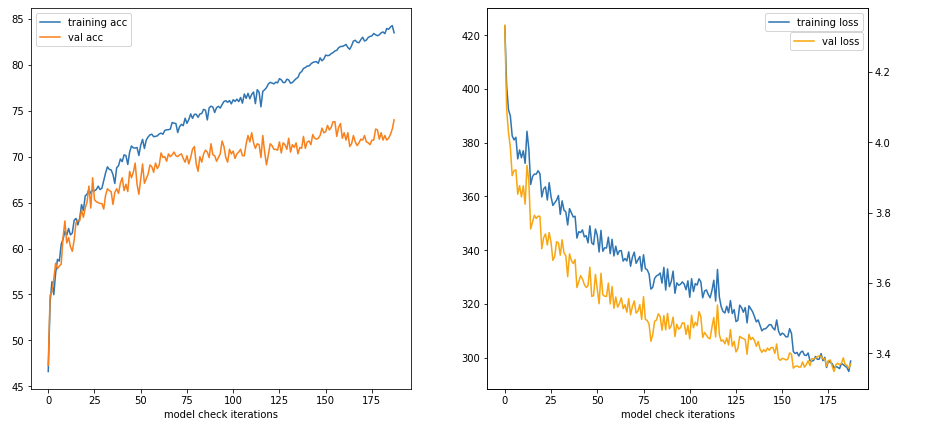
\includegraphics[scale=0.4]{rnn_best}
    \caption{Best RNN Training Curve}
    \label{fig:rnnbest}
\end{figure}

\par 
\justify
When grouped by the rnn hidden size hyperparameter, the model efficacy was not very affected, as we can see in Figure \ref{fig:rnnparams}. The hidden size controls for how much information can be encoded into the resulting hidden vectors, not enough dimensions can lead to insufficient capacity in encoding the information that we need. 

\par 
\justify
Dropout changes did significantly improve results with lower dropout rates. Drop out is effectively regularizing the network to decrease the chance of overfitting. Lower dropout rates that perform better suggests that we are not training enough before early stopping. 

\begin{figure}[h]
    \centering
    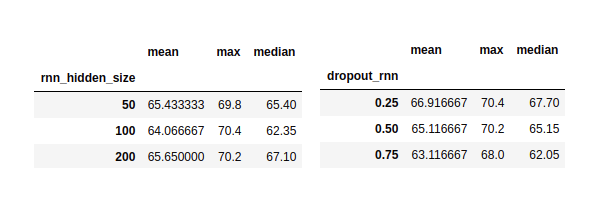
\includegraphics[scale=0.7]{rnn_params}
    \caption{RNN Accuracy by Param Groups}
    \label{fig:rnnparams}
\end{figure}


\section{CNN Hyperparameter Grid Search}
Similar to RNNs, a basic grid search was performed for CNNs over the following parameter permutations: 
\begin{itemize}
\item Learning Rate: [0.01, 0.001]
\item CNN Hidden Size: [50, 100, 200]
\item CNN Kernal Size: [3, 5, 7] (padding adjusted to keep data the same size)
\end{itemize}

\begin{figure}[h]
    \centering
    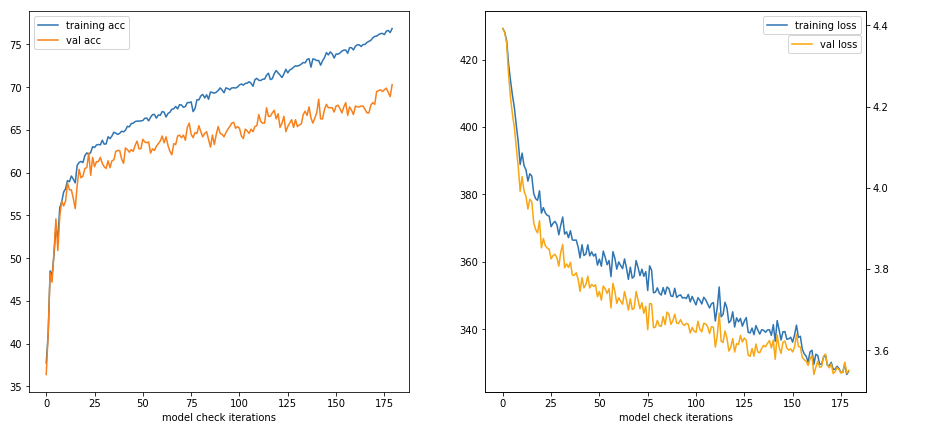
\includegraphics[scale=0.4]{cnn_best}
    \caption{Best CNN Training Curve}
    \label{fig:cnnbest}
\end{figure}


\par 
\justify
When grouped by the cnn hidden size hyperparameter, the model looks to be performing better for larger hidden size, see Figure \ref{fig:cnnparams}. At the same time, lower kernal sizes were associated with better performance. The hidden size pattern can suggest that the CNNs need more hidden size to encode the necessary information in the input sentences. While the kernal size pattern suggests either that the information is more concentrated at the 3-gram level than larger n-gram levels, or we're not training our larger kernal sizes enough for them to converge properly.


\begin{figure}[h]
    \centering
    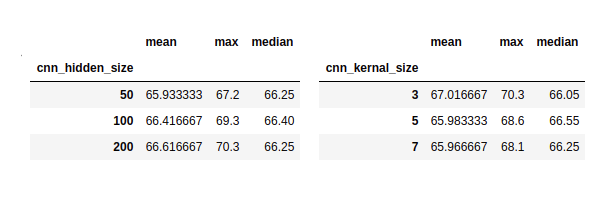
\includegraphics[scale=0.7]{cnn_params}
    \caption{CNN Accuracy by Param Groups}
    \label{fig:cnnparams}
\end{figure}

\section{MNLI Tuning}
The results for running the best RNN and the best CNN against the MNLI validation set was shown at the very top in Table \ref{tbl:mnliresults}. To further tune each genre, which had a much smaller training set, the best RNN model state\_dict was first loaded. The batch size reduced to just 32 and learning rate cut in half at the ending epoch for the previous training (recall that we use a scheduler too that decays the learning rate). Starting from the SNLI trained model, an additional 5 epochs were added to the training loop and the MNLI training set for that genre was fed to the training loop to do fine tuning. The subsequent training curve for 'fiction' is shown below in Figure \ref{fig:fictioncurve}, with the other genres similar in content. The training accuracies all improved over the additional 5 epochs and the validation accuracies capped out at a rate that was better than the SNLI trained model but worse than the training accuracy. The post MNLI tuning model at the highest validation accuracy was reported.

\par
\justify
When the post-tuned models were applied to other genres, most of them did worse for inter-genre compared to same-genre. The only exception is slate, which scored 49.7\% for the slate validation set, but 52.5\% average when applied to the other genres. This was the only result that was slightly surprising as one would expect the tuning to specifically tune the model to score better for that genre. While this was the case for most genres, slate was an outlier.

\begin{figure}[h]
    \centering
    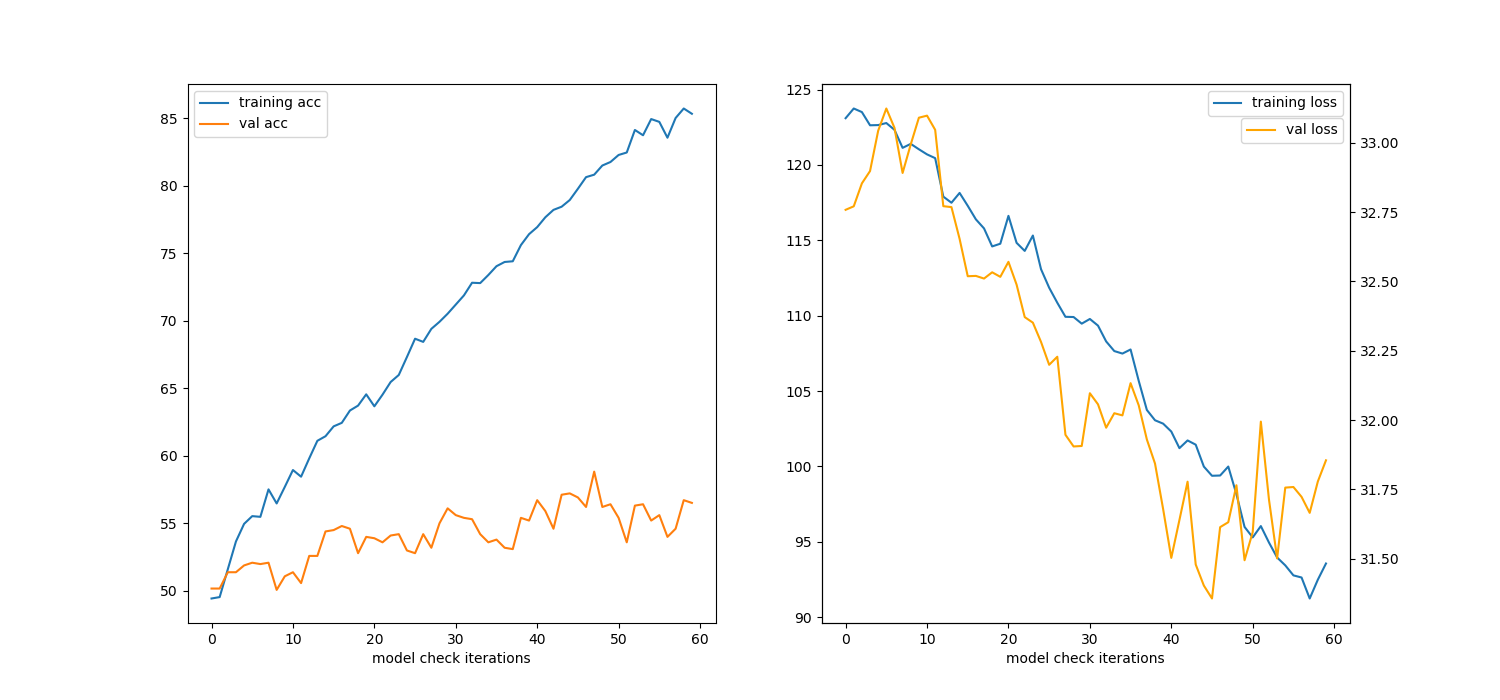
\includegraphics[scale=0.4]{fiction}
    \caption{Genre 'fiction' Training Curve}
    \label{fig:fictioncurve}
\end{figure}

\medskip

\bibliographystyle{unsrt}%Used BibTeX style is unsrt
\bibliography{refs}

\end{document}
